我们的项目是一个综合性的医疗预约管理系统,它以事件为中心,旨在为病人提供全面而便捷的医疗服务体验。该系统的架构设计采用三层结构:表示层、业务逻辑层和数据访问层,每一层都承载着特定的功能和责任。

表示层作为用户与系统之间的交互界面,不仅收集用户的输入,还展示系统的输出。为了适应不同用户的需求,我们设计了基本模式和专家模式两种不同的用户界面。在UI设计中,我们遵循了用户控制原则、减轻记忆负担原则和界面一致性原则,确保用户能够轻松、直观地操作系统。

业务逻辑层是系统的核心处理层,负责处理用户请求和执行业务逻辑。在这一层,我们细分了事件类、关系类和提醒类三个模块。事件类负责管理所有事件信息,如预约挂号和健康咨询;关系类则负责建立事件与提醒之间的联系,并定义它们之间的各种关系,例如时间或地点的关联;提醒类规定了在事件发生时应采取的行动,如发送通知或启动提醒。

数据访问层则作为系统与数据库之间的桥梁,提供数据访问接口,使得业务逻辑层能够安全、准确地读写数据库中的数据,从而确保了系统的稳定性和数据的完整性。

通过这三层结构的协同工作,我们的医疗预约管理系统能够为病人提供一站式的医疗服务,包括注册登录、查看健康信息、AI病情咨询、科室选择、预约挂号等。系统允许用户在选定的时段内选择合适的医生,极大地优化了就诊流程,提高了医疗服务的可及性和效率。此外,系统还支持电子问诊单的接收,便于病人记录和后续跟进,确保医疗服务的连续性。通过参与医疗服务评价体系,病人可以为医疗服务提供宝贵的反馈,帮助医疗机构不断改进服务质量。

在技术实现方面,我们的项目采用了面向对象的设计原则,其中前端框架的构建是我们小组的主要责任。我们选择了Vue.js作为前端框架,并使用JavaScript作为编程语言,以实现高效、响应式的用户界面。

总的来说,这些功能的实现旨在为病人提供一个无缝、高效的医疗服务体验,不仅提高了医疗服务的可及性和效率,也为医疗服务的整体改进和发展做出了贡献。


\section{经典 GoF 设计模式应用}
设计模式所提倡的⼀个原则是“相比于继承,我们更优先使用组合”。在软件工程中,设计模式是解决特定设计问题的优秀解决方案。GoF(Gang of Four)在其著作《设计模式:可复用面向对象软件的基础》~\cite{gamma2019设计模式}中提出了23种设计模式,这些模式被广泛应用于各种软件系统的开发中。本部分将探讨这些经典设计模式在我们医疗预约管理系统中的应用。

通过应用这些设计模式,我们的医疗预约管理系统能够为病人提供全面、便捷的医疗服务体验。系统支持病人注册登录、查看个人信息、向AI咨询病情、查看医院科室信息、在可选时段内选择医生进行预约挂号。此外,系统还提供账单提交和查询、费用缴纳和退费、处方查询以及搜索相关病历等功能。通过这些功能,我们旨在提高医疗服务的可及性和效率,确保病人能够轻松管理自己的医疗需求。


\subsection{创建型模式}
创建型模式主要关注对象的创建过程。通过使用这些模式,我们可以在不暴露对象创建逻辑的情况下,将对象的创建和使用分离。这样做有助于提高系统的灵活性和可维护性。

\subsubsection{工厂模式}

工厂模式是创建型模式中的一种,它提供了一种优雅的方式来创建对象。这种模式的关键在于,它通过一个统一的接口来创建对象,而具体的创建细节对客户端来说是透明的。这使得在不同的条件下,根据需求灵活地创建不同的实例成为可能。

当我们需要根据不同的条件来创建不同的对象实例时,工厂模式显得尤为有用。在这种模式下,我们通常定义一个工厂接口,然后由子类实现这个接口,并返回具体的对象。这样,对象的创建过程就被封装在子类中,而客户端代码则通过统一的接口与对象进行交互。

例如,在一个医疗预约管理系统中,我们可以设计一个名为AppointmentFactory的类\ref{app01},它根据用户的需求和医生的可用性来创建不同类型的预约对象。客户端代码可以通过这个工厂类来请求创建预约,而无需直接与具体的预约类打交道,这样就实现了创建逻辑的封装和客户端代码的简化。

\begin{figure}[htbp]
	\centering
	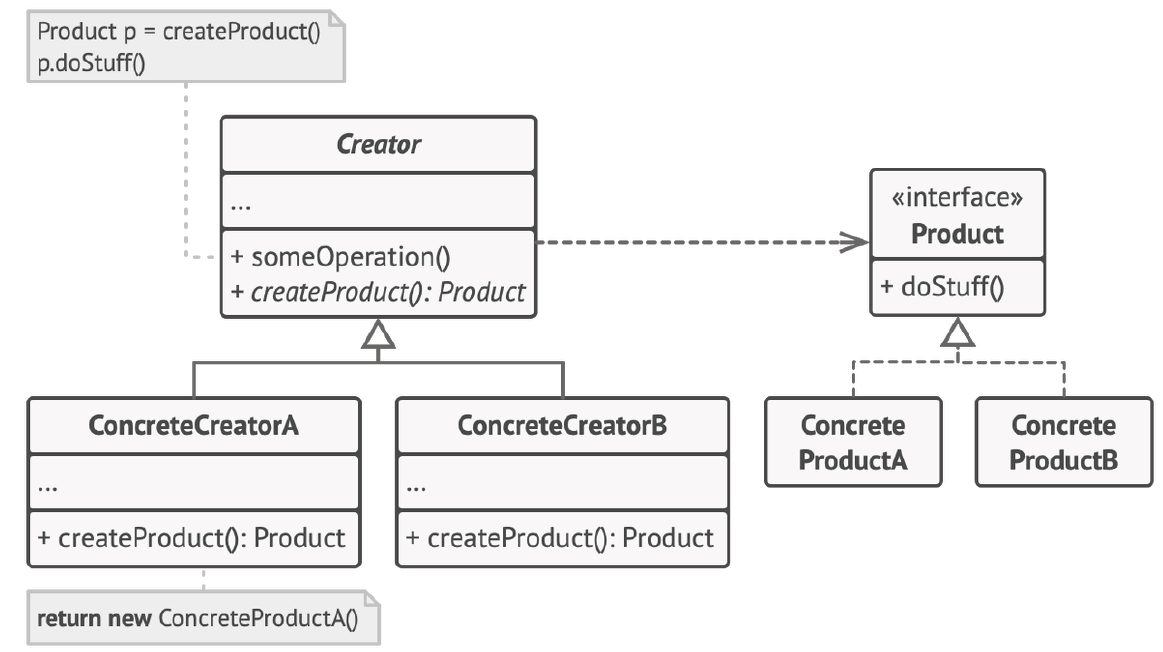
\includegraphics[width=0.6\textheight]{figures/01.png}\label{app01}
	\caption{AppointmentFactory类}
\end{figure}

通过应用工厂模式,我们的医疗预约管理系统可以更加高效地处理各种预约请求,同时保持代码的清晰和易于维护。这种模式的应用不仅提高了医疗服务的可及性和效率,也为病人提供了一个全面、便捷的医疗服务体验。病人可以通过系统轻松完成注册登录、查看个人信息、向AI咨询病情、查看医院科室信息、在可选时段内选择医生进行预约挂号等操作。

此外,系统还支持账单的提交和查询、费用的缴纳和退费、处方的查询以及相关病历的搜索等功能。通过这些功能,病人可以更好地管理自己的医疗需求,医疗机构也能够根据病人的反馈和评价来改进服务质量。这样的系统设计不仅提升了病人的满意度,也推动了医疗服务的整体改进和发展。


\subsubsection{抽象工厂}

在软件工程的众多设计模式中,抽象工厂模式(Abstract Factory Pattern)以其在创建型模式中的独特地位,为开发者提供了一种高效构建复杂对象系统的方法。该模式通过定义一个抽象的工厂接口,允许系统在不指定具体类的情况下,创建一系列相关或相互依赖的对象。这种设计哲学不仅提升了系统的灵活性和可维护性,而且简化了产品族的扩展过程,使得引入新的产品族变得简单快捷,无需修改现有的工厂类代码。

在医疗系统的背景下,抽象工厂模式的应用尤为重要。它使得系统能够灵活地创建和管理各种医疗服务对象,如不同类型的预约、提醒服务以及其他医疗相关的功能。通过定义一个抽象工厂接口,医疗系统可以生成多种预约对象和提醒方式,例如医疗预约、健康提醒等,以及相应的服务方式,如短信、邮件或应用内通知。具体的工厂类负责实现这些抽象产品的详细创建逻辑,从而在需要引入新的服务类型时,只需添加相应的具体工厂类,而无需对现有系统架构进行修改。大致如图\ref{app02}所示:
\begin{figure}[htbp]
	\centering
	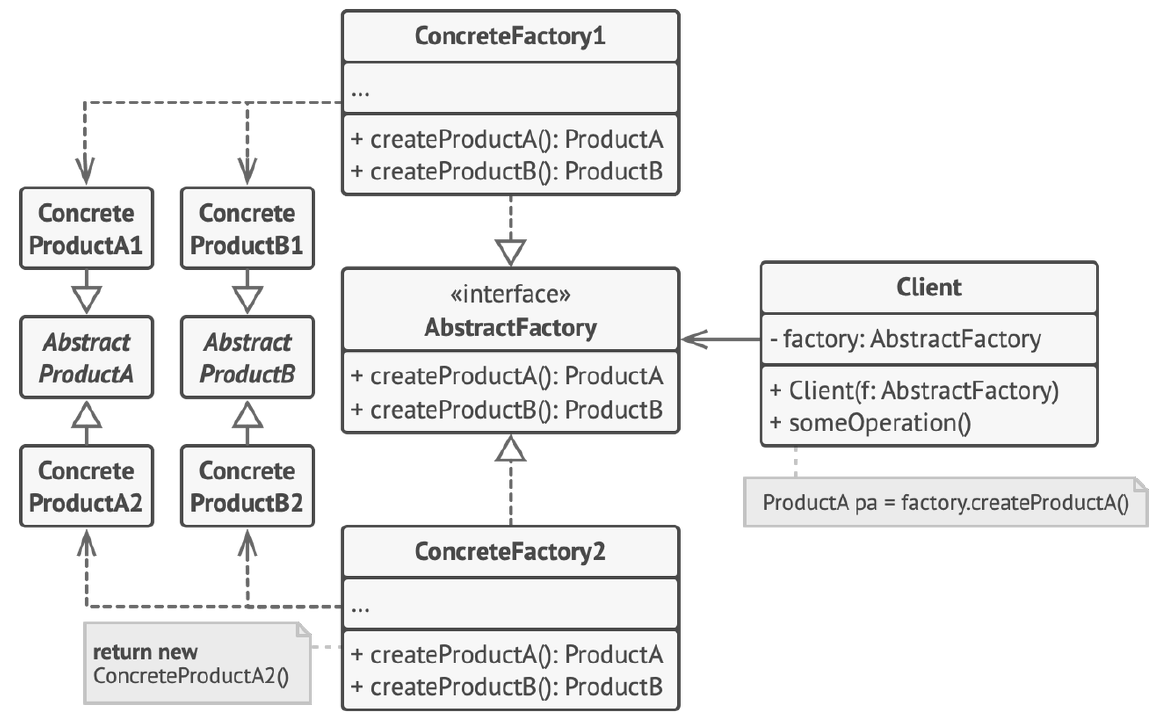
\includegraphics[width=0.6\textheight]{figures/02.png}\label{app02}
	\caption{AbstractFactory类}
\end{figure}

在医疗预约管理系统中,抽象工厂模式的应用极大地丰富了病人的医疗服务体验。系统提供了一系列的功能,包括但不限于注册登录、查看个人信息、向AI咨询病情、查看医院科室信息、在可选时段内选择医生进行预约挂号等。此外,系统还提供了账单提交和查询、费用缴纳和退费、处方查询以及相关病历搜索等功能。这些功能的实现,不仅让病人能够更加高效地管理自己的医疗需求,也为医疗机构提供了宝贵的病人反馈和评价,从而促进了服务质量的提升。

抽象工厂模式在医疗系统中的运用,不仅提升了系统的可维护性和灵活性,而且极大地丰富了用户的使用体验。通过提供一套清晰的接口和实现方式,该模式有效地支持了系统的扩展和维护,同时也为用户带来了更加直观和便捷的操作体验。这种设计使得系统不仅能够满足当前的需求,还能够灵活地适应未来的变化,从而实现长期的可持续发展。

\subsubsection{建造者模式}
在软件工程的众多设计模式中,建造者模式(Builder Pattern)以其独特的构建复杂对象的方法而著称。这种模式属于创建型模式的范畴,它通过一系列简单的对象逐步构建出一个复杂的对象。建造者模式的核心在于一个Builder类,该类负责逐步构造最终的对象,并且这个Builder类是独立于其他对象存在的。

建造者模式的主要目的是将复杂对象的构建过程与其最终表示分离开来,这样同样的构建过程就能创建出不同的表示形式。这种模式特别适用于那些由多个子对象组成的复杂对象,而这些子对象可能会因为需求变化而经常变动,但它们的组合方式却相对稳定的情况。当基本组件保持不变,而组合方式经常变化时,建造者模式就显得尤为有用,它通过分离变化和不变,使得系统更加灵活和可维护。

建造者模式的关键角色包括建造者(负责创建和提供实例)和导演(管理建造出来的实例的依赖关系)。该模式的应用实例广泛,比如肯德基在制作餐品时的流程控制,或者Java中的StringBuilder用于创建和修改字符串对象
。
\begin{figure}[htbp]
	\centering
	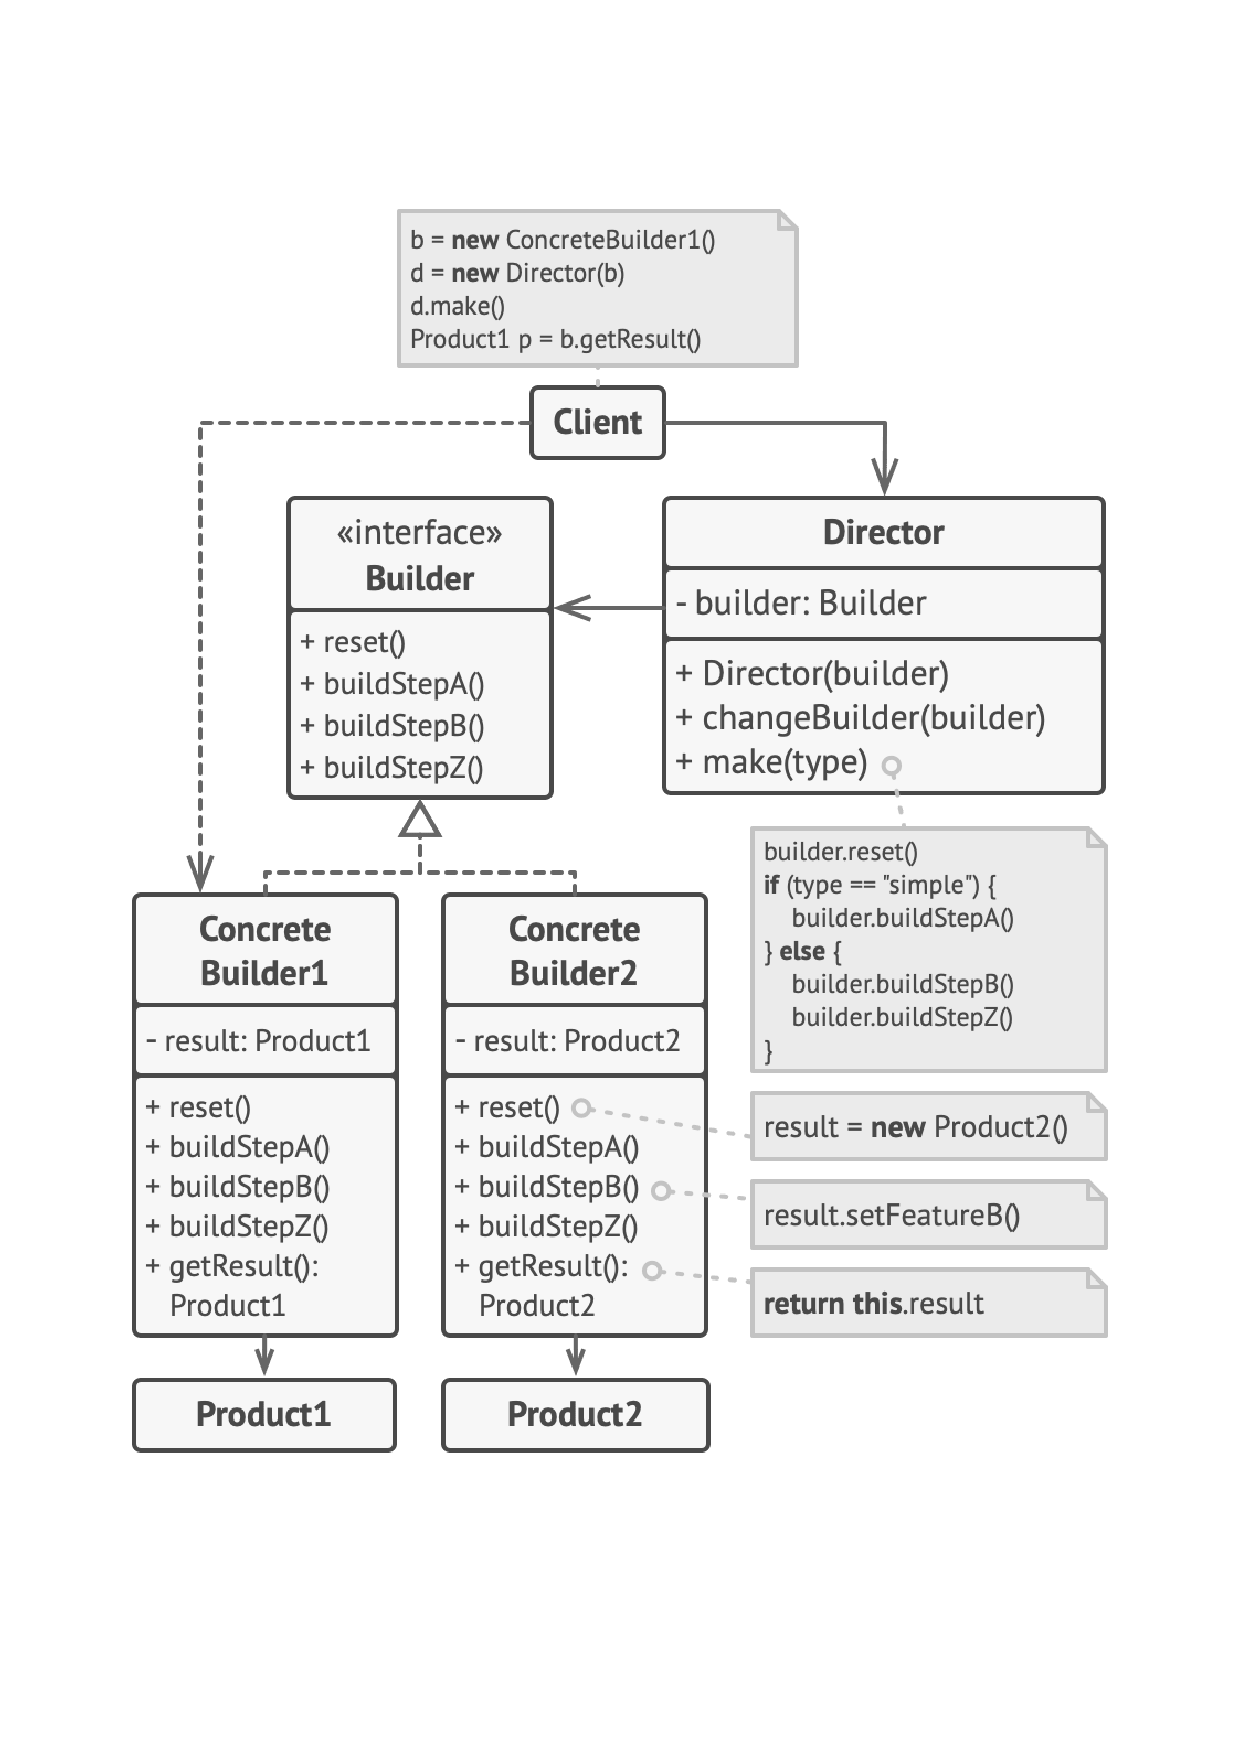
\includegraphics[width=0.5\textheight]{figures/03.pdf}\label{app03}
	\caption{Builder Pattern}
\end{figure}


建造者模式的优点在于其建造者类的独立性,易于扩展,并且能够很好地控制细节风险。然而,该模式也存在一些局限性,比如产品必须具有共同点,适用范围有限,如果内部变化复杂,则可能需要创建大量的建造类。

在使用场景上,建造者模式适用于需要生成具有复杂内部结构的对象,或者生成的对象内部属性之间存在相互依赖的情况。

与工厂模式相比,建造者模式更加关注零件装配的顺序和过程。工厂模式通常关注于对象的创建,而不涉及创建过程中的各个步骤和顺序。

在医疗系统的上下文中,建造者模式可以被用于构建复杂的医疗记录或治疗方案。例如,一个医疗记录建造者可以逐步添加病人的基本信息、病史、检查结果和治疗计划等,而治疗方案建造者则可以按照特定的治疗流程,逐步构建出包括药物处方、手术步骤和康复计划在内的复杂治疗方案。

通过这种方式,建造者模式为医疗系统提供了一种灵活且可维护的方式来构建和管理复杂的医疗数据和治疗方案,从而提高了医疗服务的质量和效率。

\subsubsection{原型模式}

在软件工程的设计模式领域中,原型模式(Prototype Pattern)是一种非常重要的创建型模式,它专注于通过复制已有对象来创建新的实例,从而提高性能和效率。这种模式特别适用于那些直接创建对象成本较高或者过程复杂的情况,例如在数据库操作之后创建对象,或者在需要频繁创建和复制对象的场景中。
\begin{figure}[htbp]
	\centering
	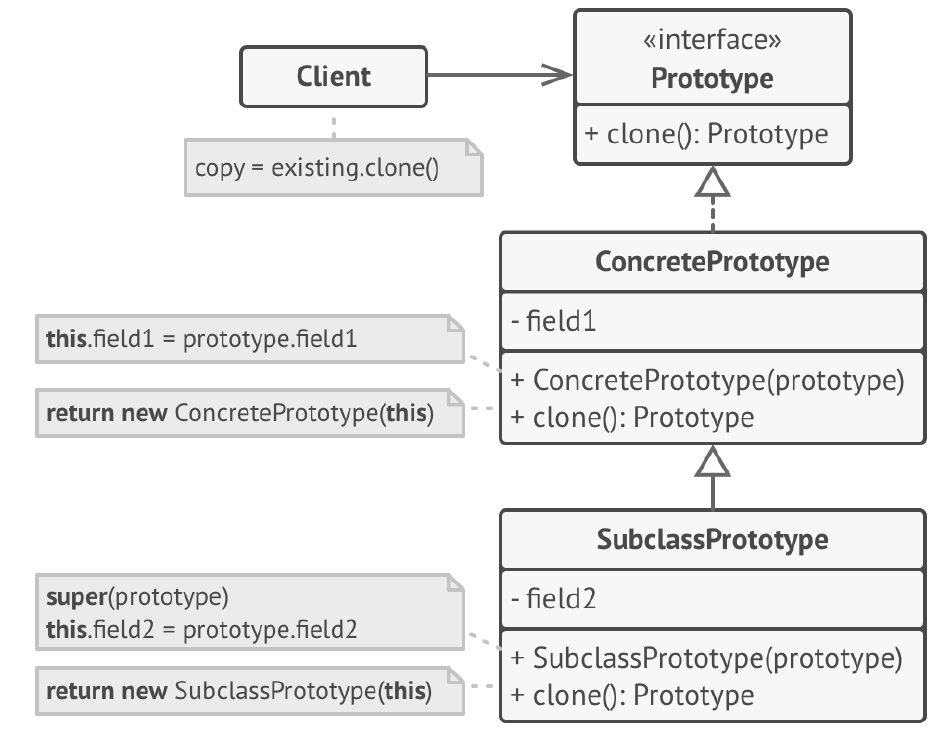
\includegraphics[width=0.5\textheight]{figures/04.png}
	\caption{Prototype Pattern}
\end{figure}
原型模式的核心思想是利用一个原型对象来生成新的实例,这样可以避免重复的构造函数调用和减少资源消耗。在实现上,可以通过实现Cloneable接口并重写clone()方法来实现对象的浅拷贝,或者通过序列化和反序列化来实现深拷贝。这种模式的优势在于它可以提高系统的性能,简化对象的创建过程,并且可以在一定程度上避免构造函数的限制。然而,它也要求开发者对类的功能进行深入的思考,确保实现Cloneable接口,并且在处理浅拷贝和深拷贝时需要特别注意。

在医疗系统中,原型模式可以发挥重要的作用。例如,在病人注册登录功能中,可以创建一个病人信息的原型对象,该对象包含了病人的基本资料、联系方式、医疗历史等信息。当有新的病人注册时,系统可以克隆这个原型对象,然后根据新病人的具体信息进行必要的修改,从而快速完成注册流程。这种方式不仅提高了注册效率,还确保了病人信息的一致性和准确性。

此外,在预约挂号功能中,原型模式同样可以大显身手。系统可以预先定义好一系列的医生排班原型对象,每个原型对象包含了医生的姓名、专业、可预约时间等信息。当病人需要预约时,系统可以克隆相应的医生排班原型对象,并根据病人的需求进行调整,如选择预约时间、医生等,从而快速完成预约流程。

在费用查询和缴纳功能中,原型模式也可以提高效率。通过创建一个费用明细的原型对象,包含费用类型、金额、日期等信息,系统可以快速生成病人的费用账单。病人或医务人员可以通过克隆这个原型对象来生成新的账单,或者对现有账单进行修改和更新。


原型模式在医疗系统中的应用可以大大提高医疗服务的效率和质量。通过快速复制和修改原型对象,系统能够为病人提供更加便捷、个性化的医疗服务,同时也减轻了医务人员的工作负担。这种模式的应用有助于构建一个高效、可靠且用户友好的医疗环境。


\subsubsection{单例模式}
在软件设计领域,单例模式(Singleton Pattern)以其简洁性和高效性而备受青睐。作为一种创建型设计模式,单例模式的核心在于确保一个类在其整个生命周期中只有一个实例存在,并且提供一个全局访问点来获取这个唯一的实例。这种模式通过将构造函数设为私有,防止外部通过new操作符创建多个实例,同时提供一个公共的静态方法,允许外部通过这个方法获取到类的唯一实例。

在实现单例模式时,需要特别注意以下几点:

1. 确保单例类在整个系统中只有一个实例。
2. 单例类需要自行创建并管理其唯一实例。
3. 单例类需要提供一个统一的访问点,供其他对象获取其实例。

单例模式的主要目的是控制类的实例化过程,确保在任何时候都只有一个实例存在,并提供一个全局访问点。这种模式特别适用于那些需要全局唯一性的场景,例如配置管理、资源池管理、日志记录等。它的优点在于能够有效地节省内存资源,避免不必要的重复创建,从而提高系统的性能。然而,单例模式也存在一些局限性,如缺乏接口、难以继承、可能与单一职责原则冲突等。

在多线程环境中,为了确保线程安全,通常在获取单例实例的方法中加入同步锁,如使用synchronized关键字或Concurrent包中的工具类来保证线程安全。

以图例形式展示该设计模式如下:
\begin{figure}[htbp]
	\centering
	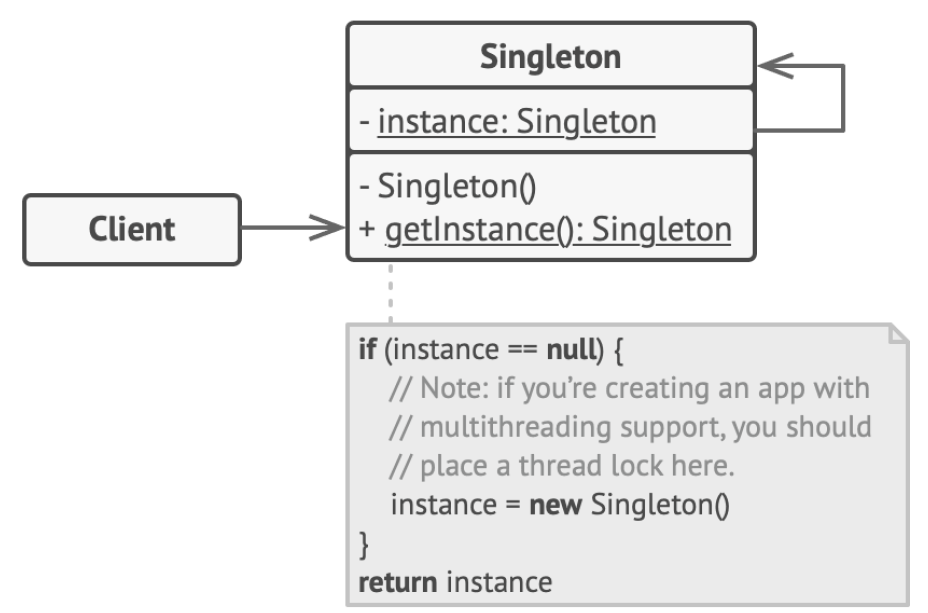
\includegraphics[width=0.5\textheight]{figures/05.png}
	\caption{Singleton Class}
\end{figure}
在医疗系统中,单例模式可以被广泛应用于提高服务的效率和质量。例如,可以创建一个全局的病人管理系统,作为单例类,管理所有病人的注册、登录、预约等信息。这样,无论在系统的哪个模块,都可以通过这个全局的病人管理系统来访问和更新病人信息,确保信息的一致性和准确性。

此外,单例模式还可以用于管理医疗资源,如医疗设备的调度和分配。通过一个全局的资源管理器,医院可以有效地监控和调配医疗资源,确保资源的合理利用和高效服务。

综上所述,单例模式在医疗系统中的应用可以极大地提升医疗服务的效率和质量,通过确保关键数据和资源的全局唯一性,为病人提供更加便捷、高效的医疗服务体验。同时,通过合理地管理资源和数据,医疗系统可以更好地满足病人的需求,提高医疗服务的可及性和效率。


\subsection{结构型模式}
\subsubsection{适配器}
在软件设计中,适配器模式(Adapter Pattern)是一种非常实用的结构型设计模式,它允许两个原本因接口不兼容而无法一起工作的类相互合作。这种模式通过引入一个适配器类,将一个类的接口转换成客户期望的另一个接口,从而使得原本不兼容的类能够无缝集成。

在医疗系统的上下文中,适配器模式可以发挥重要作用,特别是在需要与多个不同的医疗信息系统或设备进行交互时。例如,一个医疗预约系统可能需要与各种不同的医疗日历应用程序进行通信,以便在用户设定的特定时间和日期发送提醒。这些应用程序可能具有不同的API定义,导致它们之间的接口不兼容,从而使得医疗预约系统难以直接与它们进行交互。

为了解决这一问题,我们可以利用适配器模式来创建一个适配器层,将医疗预约系统的统一接口转换为特定日历应用程序的接口。适配器对象将充当桥梁,将医疗预约系统的请求转换为各个日历应用程序能够理解的特定API调用,并将结果反馈回医疗预约系统。

以下是一个简化的代码示例,展示了如何使用适配器模式来实现这一功能:

\definecolor{codegreen}{rgb}{0,0.6,0}
\definecolor{codegray}{rgb}{0.5,0.5,0.5}
\definecolor{codepurple}{rgb}{0.58,0,0.82}
\definecolor{backcolour}{rgb}{0.95,0.95,0.92}

\lstdefinestyle{mystyle}{
	backgroundcolor=\color{backcolour},
	commentstyle=\color{codegreen},
	keywordstyle=\color{magenta},
	numberstyle=\tiny\color{codegray},
	stringstyle=\color{codepurple},
	basicstyle=\ttfamily\footnotesize,
	breakatwhitespace=false,
	breaklines=true,
	captionpos=b,
	keepspaces=true,
	numbers=left,
	numbersep=5pt,
	showspaces=false,
	showstringspaces=false,
	showtabs=false,
	tabsize=2,
	language=Java,
	frame=none,
	columns=fullflexible,
	showstringspaces=false,
	xleftmargin=0.5cm
}

\lstset{style=mystyle}

\begin{lstlisting}[caption={医疗预约系统期望的统一事件提醒接口}]
	// 患者信息系统期望的统一医疗设备接口
	interface MedicalDevice {
		void integrateData(String patientId, String data);
	}
	
	// 某型号X光机的接口
	interface XrayMachine {
		void receiveImage(String patientId, byte[] image);
	}
	
	// 某型号心电图机的接口
	interface ECGMachine {
		void receiveReadings(String patientId, int[] readings);
	}
	
	// X光机适配器类,将X光机接口转换为统一医疗设备接口
	class XrayAdapter implements MedicalDevice {
		private XrayMachine xrayMachine;
		
		public XrayAdapter(XrayMachine xrayMachine) {
			this.xrayMachine = xrayMachine;
		}
		
		@Override
		public void integrateData(String patientId, String data) {
			// 假设data是转换后的图像数据
			byte[] image = convertDataToImage(data);
			xrayMachine.receiveImage(patientId, image);
		}
	}
	
	// 心电图机适配器类,将心电图机接口转换为统一医疗设备接口
	class ECGAdapter implements MedicalDevice {
		private ECGMachine ecgMachine;
		
		public ECGAdapter(ECGMachine ecgMachine) {
			this.ecgMachine = ecgMachine;
		}
		
		@Override
		public void integrateData(String patientId, String data) {
			// 假设data是转换后的心电图读数
			int[] readings = convertDataToReadings(data);
			ecgMachine.receiveReadings(patientId, readings);
		}
	}
\end{lstlisting}

通过这种方式,患者信息系统可以通过统一的接口与不同的医疗设备进行交互,而无需关心具体的设备细节。这种灵活性使得系统能够轻松集成新的医疗设备,只需提供相应的适配器类即可。

在医疗系统中,适配器模式的应用可以极大地提高系统的互操作性和可扩展性,使得系统能够更好地服务于病人和医务人员。例如,除了医疗设备集成外,适配器模式还可以用于患者管理系统、医疗信息系统、药品库存管理等多个方面,确保不同系统和设备之间的顺畅通信和数据交换。通过这种方式,医疗系统能够为病人提供一个全面、便捷的医疗服务体验,从而提高医疗服务的可及性和效率。


\subsubsection{桥接器}


在软件设计领域,桥接模式(Bridge Pattern)是一种结构型设计模式,它允许将抽象与实现分离,使得两者可以独立地变化。这种模式特别适用于那些需要将一个大类或一系列紧密相关的类拆分为两个独立层次结构的场景,以便在开发过程中分别进行使用和扩展。

在医疗系统中,桥接模式可以用于实现病人服务的多样化和灵活性。例如,医疗系统可能需要支持多种不同类型的事件提醒,如弹出窗口提醒、发送短信、发送电子邮件等,同时也需要支持多种不同类型的事件,如预约提醒、检查结果通知、健康教育信息等。如果直接采用继承的方式来实现这些功能,随着事件类型和提醒方式的增加,将会导致类的数量急剧增加,从而增加了代码的复杂度和耦合度。

通过使用桥接模式,我们可以将事件提醒的抽象部分(定义事件的基本属性和行为)与实现部分(具体提醒的方式)分离开来。抽象部分可以定义一个包含实现部分引用的接口,而实现部分则负责具体的提醒逻辑。这样,当需要增加新的事件类型或提醒方式时,只需添加相应的实现类即可,而无需修改现有的抽象类或其他实现类。

在医疗系统的具体应用中,桥接模式可以帮助我们构建一个灵活的事件提醒系统。例如,可以将事件分为普通事件和特殊事件,同时根据事件的性质进一步将其细分为时间相关事件和地点相关事件。通过桥接模式,我们可以为每种事件类型和每个维度创建相应的实现类,而这些类之间不会相互影响,从而使得整个系统更加模块化和易于维护。

\begin{lstlisting}[caption={桥接模式来实现医疗系统中的事件提醒功能}]
// 事件抽象部分的接口
interface Event {
	void notify();
}

// 普通事件的实现
class RegularEvent implements Event {
	private String message;
	
	public RegularEvent(String message) {
		this.message = message;
	}
	
	@Override
	public void notify() {
		System.out.println("Regular event: " + message);
	}
}

// 特殊事件的实现
class SpecialEvent implements Event {
	private String message;
	
	public SpecialEvent(String message) {
		this.message = message;
	}
	
	@Override
	public void notify() {
		System.out.println("Special event: " + message);
	}
}

// 事件提醒实现部分的接口
interface Notification {
	void send();
}

// 短信提醒的实现
class SMSNotification implements Notification {
	private Event event;
	
	public SMSNotification(Event event) {
		this.event = event;
	}
	
	@Override
	public void send() {
		System.out.println("Sending SMS notification for event: " + event.notify());
	}
}

// 电子邮件提醒的实现
class EmailNotification implements Notification {
	private Event event;
	
	public EmailNotification(Event event) {
		this.event = event;
	}
	
	@Override
	public void send() {
		System.out.println("Sending email notification for event: " + event.notify());
	}
}
\end{lstlisting}
通过这种方式,医疗系统可以根据病人的需求灵活地选择不同类型的事件和提醒方式,同时保持代码的清晰和系统的可维护性。这种设计不仅提高了系统的扩展性,也使得未来的维护和升级变得更加容易。

类图大致如下:

\begin{figure}[htbp]
	\centering
	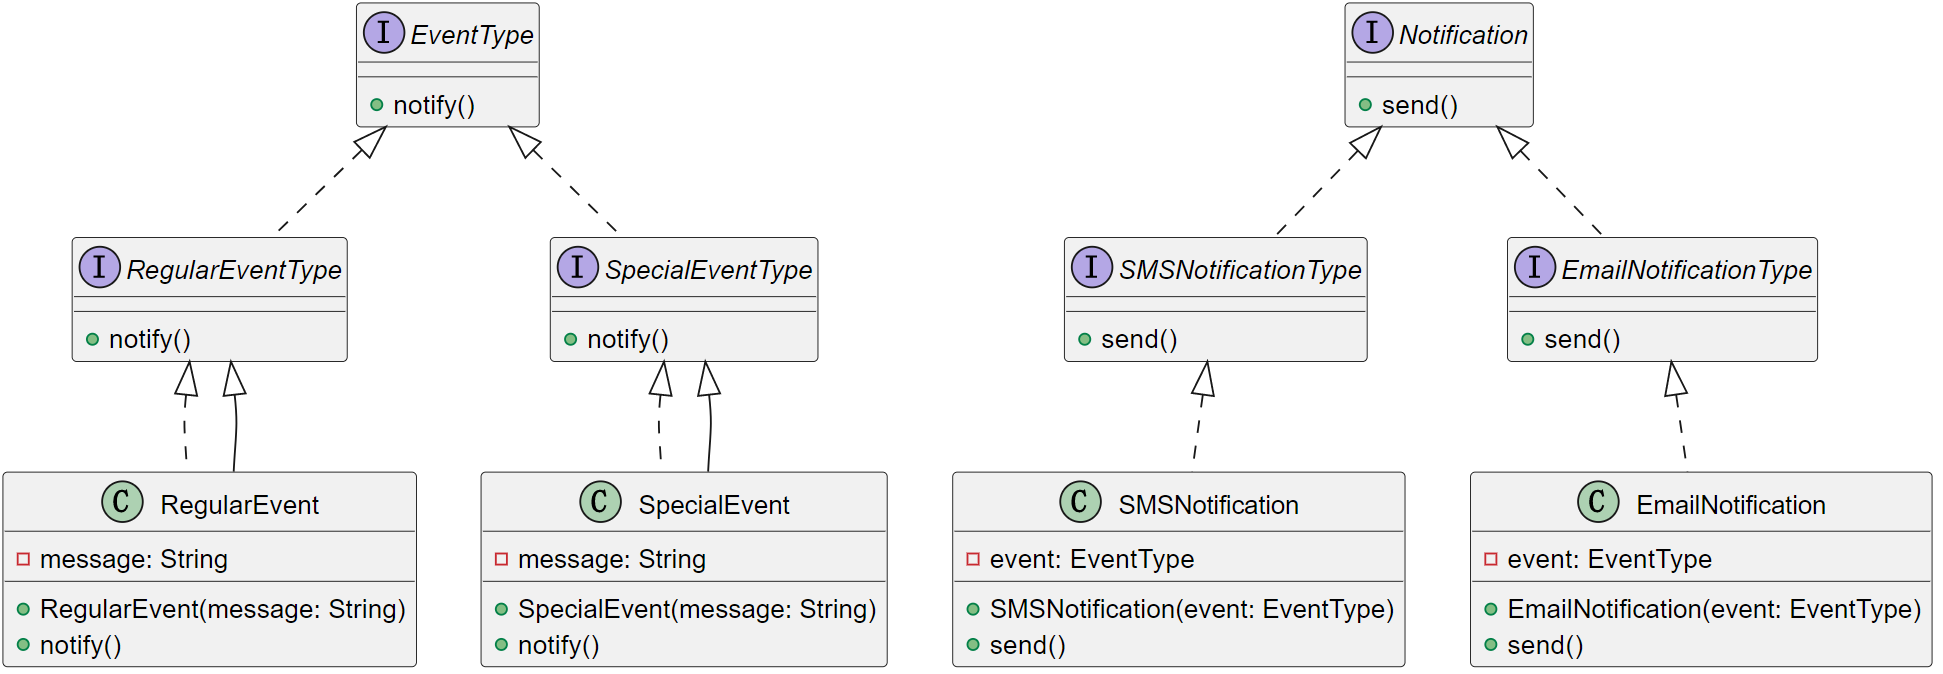
\includegraphics[width=0.6\textheight]{figures/07.png}
	\caption{桥接模式的类图}
\end{figure}


在重构后的类图中,我们采用了桥接模式来优化设计。通过这种方式,我们将事件的普通性或特殊性这一属性独立出来,并用一个新的接口来表示。这种改变显著降低了原有继承体系的耦合度,并且简化了类的结构。通过观察新的类图,我们可以清晰地看到,类之间的关系变得更加清晰,系统的可维护性和可扩展性得到了显著提升。


\begin{figure}[htbp]
	\centering
	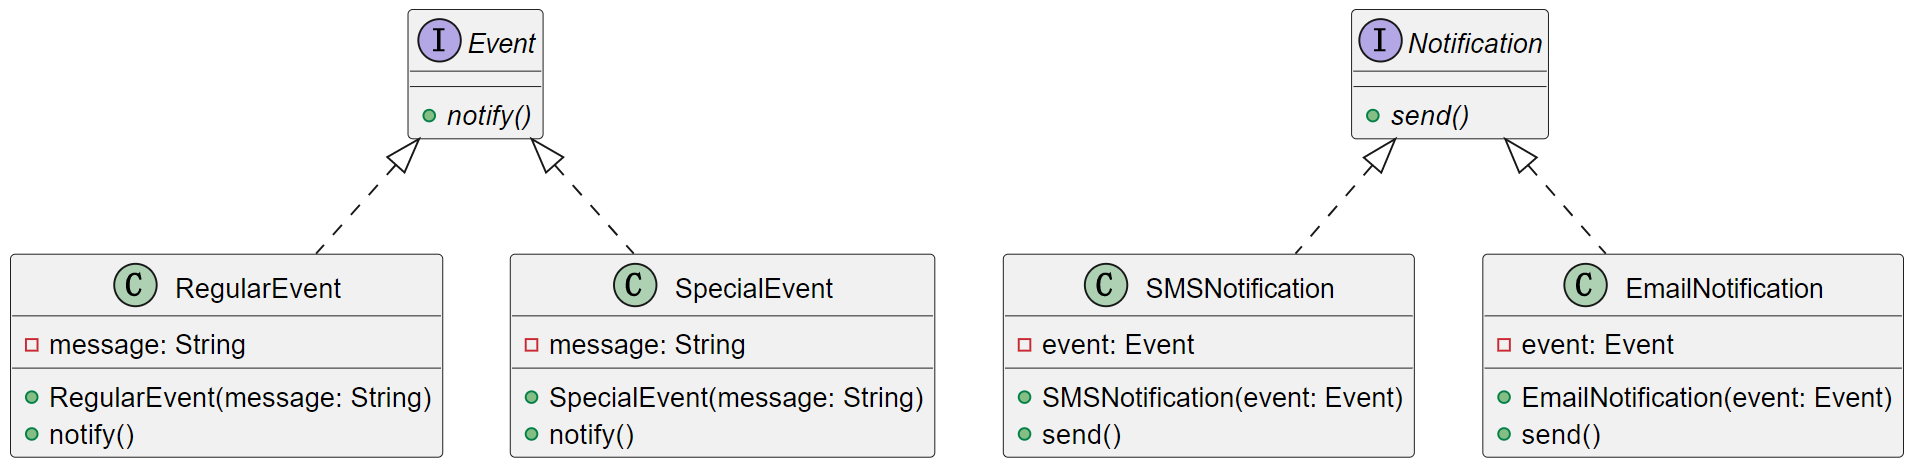
\includegraphics[width=0.6\textheight]{figures/06.png}
	\caption{优化后的桥接模式的类图}
\end{figure}

\subsubsection{外观}

在软件设计中,外观模式(Facade Pattern)是一种结构型设计模式,它通过提供一个简化的接口来封装复杂的子系统。这种模式的目的是为子系统的一组复杂接口提供一个统一的高层接口,从而降低了系统的复杂性,并使得子系统更加易于使用。

外观模式在处理复杂的系统时尤为有用,例如在医疗信息系统中,可能存在多个子系统来处理不同的任务,如病人信息管理、预约系统、费用计算等。这些子系统可能具有复杂的接口和多个交互点,使得客户端代码难以理解和使用。在这种情况下,外观模式可以提供一个统一的外观类(Facade Class),它将所有的子系统操作封装在一个简单的接口后面。

在医疗预约系统中,外观模式可以用于创建一个统一的接口,用于管理病人的预约、咨询、费用支付等操作。例如,一个外观类可以提供如下方法:

\begin{lstlisting}[caption={外观类}]
public class MedicalFacade {
	private PatientManagementSystem patientManagement;
	private AppointmentSystem appointmentSystem;
	private BillingSystem billingSystem;
	
	public MedicalFacade() {
		patientManagement = new PatientManagementSystem();
		appointmentSystem = new AppointmentSystem();
		billingSystem = new BillingSystem();
	}
	
	public void registerPatient(String name, String idNumber) {
		patientManagement.registerPatient(name, idNumber);
	}
	
	public void bookAppointment(String patientId, String doctorId, String date) {
		appointmentSystem.bookAppointment(patientId, doctorId, date);
	}
	
	public void payBill(String patientId, double amount) {
		billingSystem.collectPayment(patientId, amount);
	}
	
	// 其他简化的医疗服务操作...
}
\end{lstlisting}

通过这个外观类,客户端代码可以轻松地执行复杂的操作,而无需了解背后子系统的具体实现。这不仅简化了客户端代码的开发,也使得系统更易于维护和扩展。

在实际应用中,外观模式有助于为病人提供一个全面、便捷的医疗服务体验。例如,病人可以通过一个简单的界面来注册、登录、查询基本信息、向AI咨询病情、查看医院科室信息、选择医生并预约挂号、提交和查看账单、缴纳费用以及查询处方和搜索相关病历。外观模式使得这些功能背后的复杂性被隐藏,病人只需通过一个简单直观的界面来完成所有操作,从而提高了医疗服务的可及性和效率。

\subsubsection{代理}
在软件架构设计中,代理模式(Proxy Pattern)是一种结构型设计模式,它允许创建一个代理对象,作为原对象的占位符或替代品。代理模式的关键在于,代理对象控制着对原对象的访问,并有能力在将请求转发给原对象前后进行额外的处理工作。这种模式在软件工程中有广泛的应用,例如在数据库连接池管理、远程服务调用、缓存机制、日志记录等方面。特别地,Spring框架利用代理模式实现了其面向切面编程(AOP)的功能。

面向切面编程是一种编程范式,它允许开发者将具有横切性质的代码与主要业务逻辑分离,使得这些代码能够更加模块化和松耦合。通过AOP,可以实现诸如日志记录、安全性检查、事务管理等功能,而无需在每个相关模块中重复编写相同的代码。Spring AOP通过代理模式实现了这一点,提供了基于JDK动态代理和基于CGLib的两种代理机制。基于JDK的动态代理要求目标对象实现至少一个接口,而CGLib代理则不要求目标对象实现接口,可以代理任何类。

在Spring AOP中,通过定义切面(Aspect)来实现横切关注点的模块化。切面由通知(Advice)和切点(Pointcut)组成。通知定义了切面在何处以及如何执行,而切点则指定了哪些方法或类应该被通知所增强。当目标对象的方法被调用时,Spring容器会自动创建一个代理对象,并将切面逻辑应用到该代理对象上。

代理模式不仅为AOP提供了实现的基础,还可以在多种场景下单独使用,例如远程服务代理、虚拟代理、延迟加载等。在事件提醒小助手的应用中,代理模式可以用来控制对提醒功能的访问,并在访问过程中增加额外的逻辑,如权限验证、日志记录、异常处理等。

具体到实现过程,可以按照以下步骤操作:

1. 定义提醒功能的目标对象,并为其创建一个接口,如`ReminderInterface`,包含必要的方法,如添加、修改和删除提醒事件。

2. 创建目标对象的代理类`ReminderProxy`,该类实现`ReminderInterface`,并持有目标对象的引用。

3. 在代理类中,根据需要在目标对象的方法调用前后添加额外的处理逻辑。

4. 通过代理对象来访问提醒功能,而不是直接访问目标对象。

5. 代理对象确保只有经过验证的用户才能执行添加、修改或删除提醒事件的操作,从而保障了提醒功能的安全性。


通过应用代理模式,事件提醒小助手不仅能够确保提醒事件的安全性和完整性,还能够提高服务的效率和质量,为病人提供全面、便捷的医疗服务体验。这包括病人注册登录、查看个人信息、向AI咨询病情、查看医院科室信息、在可选时段内选择医生进行预约挂号、提交和查询账单、缴纳费用、查询处方以及搜索相关病历等功能。通过这些功能,病人可以更加轻松地管理自己的医疗需求,享受到更加高效和个性化的医疗服务。

\subsection{行为模式}
\subsubsection{迭代器}
在软件设计中,行为模式是一类重要的设计模式,它们专注于对象之间的通信。在这些行为模式中,迭代器模式(Iterator Pattern)扮演着至关重要的角色,它允许开发者在不暴露其底层数据结构的情况下,顺序访问一个聚合对象中的元素。这种模式通过将遍历逻辑封装在一个迭代器对象中,从而使得遍历过程与聚合对象的内部结构解耦,提高了代码的灵活性和可维护性。

迭代器模式的核心思想是定义一个迭代器接口,该接口包含用于遍历集合的方法,如`next()`用于获取下一个元素,`hasNext()`用于检查是否还有更多元素。客户端代码通过这个统一的接口与迭代器交互,而无需关心集合的具体实现细节,如列表、栈、树等。这种设计使得客户端可以轻松地遍历任何类型的集合,只要这些集合提供了相应的迭代器实现。

在医疗信息系统中,迭代器模式可以用于实现对病人信息、医生排班、预约记录等数据集合的有效遍历。例如,一个医院可能需要对病人的病历进行分析,以便提供更好的医疗服务。通过使用迭代器模式,系统可以提供一个统一的接口来遍历所有病人的病历记录,而无需关心这些记录是如何存储和组织的。

具体到实现,医疗信息系统可以定义一个`PatientRecordIterator`接口,该接口包含`next()`和`hasNext()`方法。然后,针对不同类型的数据集合,如数据库中的病人记录表、文件系统中的病历文档等,系统可以提供具体的迭代器实现。这些迭代器负责跟踪遍历进度,并在客户端请求时提供相应的病历数据。

此外,迭代器模式还允许多个迭代器独立地遍历同一个集合。这意味着,不同的医疗服务人员可以同时访问和分析病人的病历数据,而不会相互干扰。这种特性对于提高医疗信息系统的效率和响应速度至关重要。

综上所述,迭代器模式在医疗信息系统中的应用,不仅提高了数据遍历的效率和灵活性,而且为病人提供了全面、便捷的医疗服务体验。通过这种方式,医疗系统能够更好地管理病人信息,优化资源分配,并提高医疗服务的整体质量。

\subsubsection{中介者}

在设计软件系统时,中介者模式(Mediator Pattern)是一种行为型设计模式,它允许多个对象之间的交互通过一个中介对象进行,而不是让这些对象直接相互引用。这种模式的目的是减少对象之间的耦合,使得系统更加灵活和易于维护。

在医疗信息系统中,中介者模式可以用于协调不同组件之间的通信,例如事件管理、提醒服务和时间调度等。通过使用中介者模式,我们可以创建一个中央组件(即中介者),它负责处理各个子系统之间的交互,而不是让这些子系统直接相互通信。

以下是一个简化的代码示例,展示了如何在医疗信息系统中应用中介者模式:

\begin{lstlisting}[caption={中介者}]
class Event {
	private String name;
	private String date;
	private String time;
	private Reminder reminder;
	
	public Event(String name, String date, String time) {
		this.name = name;
		this.date = date;
		this.time = time;
		this.reminder = null;
	}
	
	public void addReminder(Reminder reminder) {
		this.reminder = reminder;
	}
	
	public void cancel() {
		if (this.reminder != null) {
			this.reminder.cancel();
		}
	}
}

class Reminder {
	private Event event;
	private String time;
	
	public Reminder(Event event, String time) {
		this.event = event;
		this.time = time;
	}
	
	public void notifyReminder() {
		System.out.println("Reminder: " + event.getName() + " at " + event.getDate() + ", " + time);
	}
	
	public void cancel() {
		System.out.println("Cancelled reminder: " + event.getName() + " at " + event.getDate() + ", " + time);
	}
}

class Mediator {
	private List<Event> events;
	
	public Mediator() {
		this.events = new ArrayList<>();
	}
	
	public void addEvent(Event event) {
		this.events.add(event);
	}
	
	public void start() {
		while (true) {
			String currentTime = getCurrentTime(); // Assume implementation of getCurrentTime()
			for (Event event : events) {
				if (event.getTime().equals(currentTime)) {
					event.getReminder().notifyReminder();
				}
			}
		}
	}
}

public class Main {
	public static void main(String[] args) {
		// 创建中介者对象
		Mediator mediator = new Mediator();
		
		// 创建事件对象
		Event event1 = new Event("Consultation", "2024-04-15", "09:30");
		Event event2 = new Event("Surgery", "2024-04-16", "14:00");
		
		// 创建提醒对象
		Reminder reminder1 = new Reminder(event1, "09:30");
		Reminder reminder2 = new Reminder(event2, "14:00");
		
		// 将提醒添加到事件中
		event1.addReminder(reminder1);
		event2.addReminder(reminder2);
		
		// 将事件添加到中介者中
		mediator.addEvent(event1);
		mediator.addEvent(event2);
		
		// 启动中介者组件
		mediator.start();
	}
}
\end{lstlisting}
UML图为:
\begin{figure}[htbp]
	\centering
	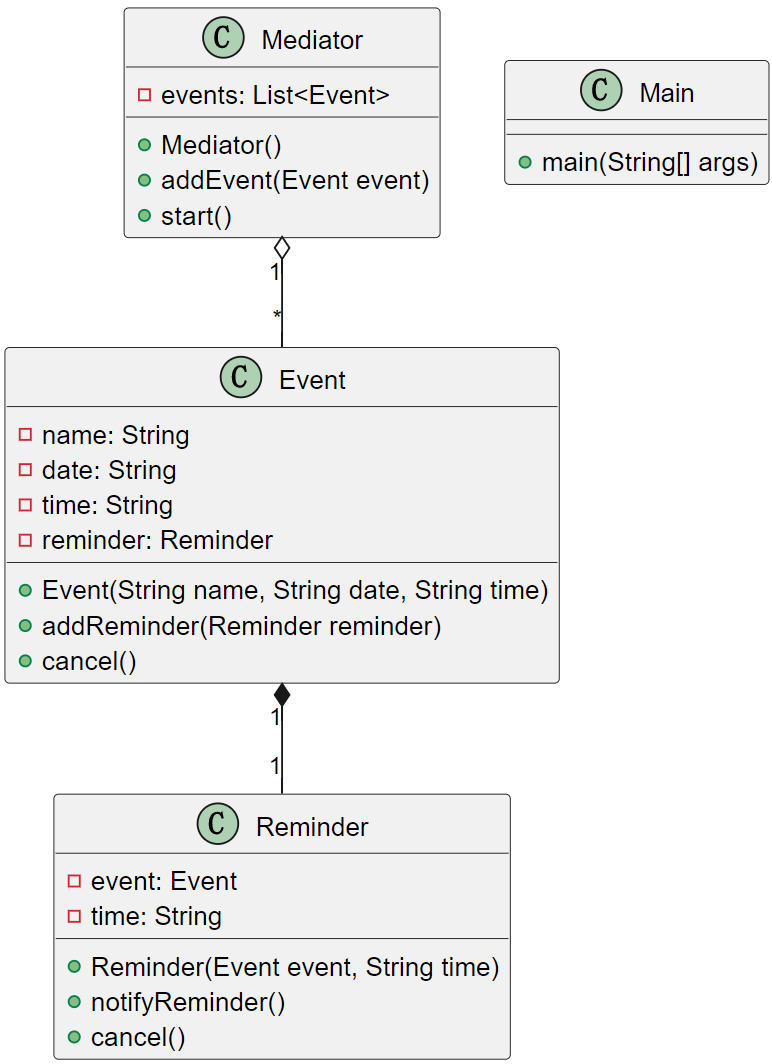
\includegraphics[width=0.3\textheight]{figures/14.png}
	\caption{Builder Pattern}
\end{figure}
在这个例子中,`Mediator`类作为中介者,负责管理`Event`对象的集合,并在指定的时间触发提醒。`Event`对象不再直接与`Reminder`对象交互,而是通过中介者来协调。这样,当需要修改提醒逻辑或添加新的事件类型时,我们只需关注中介者组件,而无需修改事件或提醒的代码。

中介者模式在医疗信息系统中的应用,可以提高系统的可维护性和扩展性,使得添加新功能或修改现有功能变得更加容易。此外,这种模式还有助于简化系统架构,因为所有的交互都通过一个中介者进行,而不是让各个组件直接相互通信,从而降低了系统的整体复杂性。

通过中介者模式,医疗信息系统可以为病人提供更加全面和便捷的服务,如预约挂号、查询医生排班、接收预约提醒等。同时,系统还能够高效地处理费用查询、缴费退费、处方查询和病历搜索等事务,确保病人能够及时接收到所需的医疗服务,提高医疗服务的可及性和效率。

\subsubsection{观察者}
在软件工程的行为设计模式中,观察者模式(Observer Pattern)是一种允许对象之间的松耦合设计的方法。该模式通过定义对象之间的一对多依赖关系,使得当一个对象的状态发生变化时,所有依赖于它的对象都会得到通知并自动更新。

在医疗信息系统的上下文中,观察者模式可以用于实现一个高效的事件通知和处理机制。例如,当病人的预约状态发生变化,或者医生的排班表更新时,相关的系统组件,如提醒服务、日程安排、费用结算等,都需要得到通知并作出相应的调整。通过应用观察者模式,我们可以确保所有相关的对象都能够及时响应状态的变化,从而提供连贯和一致的医疗服务体验。

具体来说,我们可以定义一个主题接口(Subject),它包含了添加观察者(attach)、移除观察者(detach)和通知所有观察者(notify)的方法。事件类(Event)作为具体的主题实现,负责管理其状态,并在状态发生变化时通知所有注册的观察者。提醒类(Reminder)和闹钟类(Alarm)作为观察者(Observer)的角色,实现了更新接口(update),以便在接收到事件通知时能够做出适当的反应。

以下是一个简化的代码示例,展示了如何在医疗信息系统中应用观察者模式:

\begin{lstlisting}[caption={观察者例子}]
% 主题接口
interface Subject {
	void attach(Observer observer);
	void detach(Observer observer);
	void notifyObservers();
}

% 具体的主题实现:事件类
class Event implements Subject {
	private List<Observer> observers = new ArrayList<>();
	private String status;
	
	public void setStatus(String status) {
		this.status = status;
		notifyObservers();
	}
	
	@Override
	public void attach(Observer observer) {
		observers.add(observer);
	}
	
	@Override
	public void detach(Observer observer) {
		observers.remove(observer);
	}
	
	@Override
	public void notifyObservers() {
		for (Observer observer : observers) {
			observer.update(this);
		}
	}
}

% 观察者接口
interface Observer {
	void update(Subject subject);
}

% 具体观察者实现:提醒类
class Reminder implements Observer {
	@Override
	public void update(Subject subject) {
		Event event = (Event) subject;
		// 更新提醒信息
		System.out.println("Reminder: " + event.getStatus());
	}
}

% 具体观察者实现:闹钟类
class Alarm implements Observer {
	@Override
	public void update(Subject subject) {
		Event event = (Event) subject;
		// 设置闹钟
		System.out.println("Alarm set for: " + event.getStatus());
	}
}

% 客户端代码
public class HospitalSystem {
	public static void main(String[] args) {
		Event event = new Event();
		Reminder reminder = new Reminder();
		Alarm alarm = new Alarm();
		
		event.attach(reminder);
		event.attach(alarm);
		
		// 模拟状态变化
		event.setStatus("Doctor's appointment scheduled.");
	}
}

\end{lstlisting}
UML图为:
\begin{figure}[htbp]
	\centering
	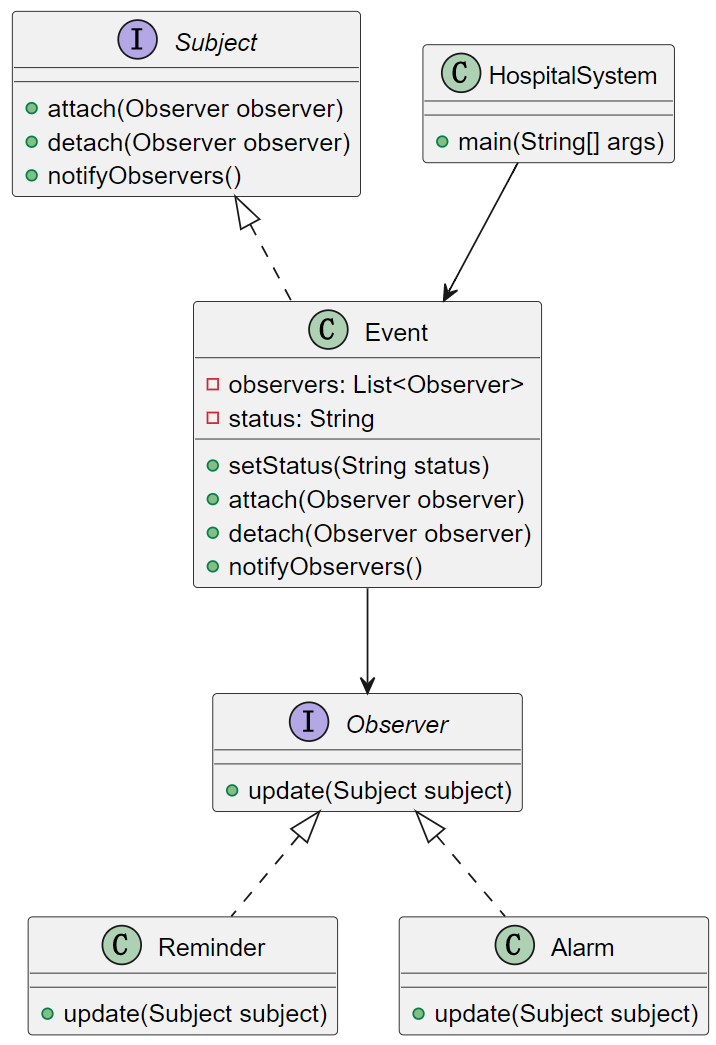
\includegraphics[width=0.3\textheight]{figures/13.png}
	\caption{Builder Pattern}
\end{figure}
在这个例子中,当事件状态发生变化时,所有注册的观察者(提醒和闹钟)都会收到通知,并执行相应的更新操作。这种设计使得医疗信息系统能够灵活地响应各种状态变化,确保病人能够及时接收到预约提醒和日程安排,从而提高医疗服务的可及性和效率。

通过观察者模式,医疗信息系统可以为病人提供更加全面和便捷的服务,包括预约挂号、查询医生排班、接收预约提醒、查看费用账单、缴纳医疗费用、查询处方信息和搜索相关病历等。同时,系统还能够高效地处理退号、退费等操作,确保病人能够享受到连贯一致的医疗服务体验。

\subsubsection{状态}
在软件设计领域,状态模式(State Pattern)是一种行为型设计模式,它允许对象在其内部状态改变时改变其行为。这种模式特别适用于对象的行为取决于其状态,并且它必须在运行时根据状态改变其行为的情况。状态模式通过将特定状态的行为封装在独立的类中,从而使得状态的转换变得简单且易于管理。

在医疗信息系统中,状态模式可以用来管理病人预约的不同状态,例如预约的创建、确认、提醒、完成和取消等。每个状态都对应一个特定的类,这些类实现了具体的状态行为。上下文对象,即预约对象,持有一个当前状态对象的引用,并将所有与状态相关的行为委托给该状态对象。当状态发生变化时,上下文对象只需切换到对应状态的类实例,而无需修改自身的代码。

以下是一个简化的代码示例,展示了如何在医疗信息系统中应用状态模式来管理预约状态:
\begin{lstlisting}[caption={状态例子}]
% 状态接口
interface State {
	void handle();
}

% 具体状态类:预约创建
class CreatedState implements State {
	@Override
	public void handle() {
		// 处理预约创建
		System.out.println("Appointment created. Awaiting confirmation.");
	}
}

% 具体状态类:预约确认
class ConfirmedState implements State {
	@Override
	public void handle() {
		// 处理预约确认
		System.out.println("Appointment confirmed. Reminder will be sent.");
	}
}

% ... 其他状态类

% 上下文类:预约对象
class Appointment {
	private State state;
	
	public void setState(State state) {
		this.state = state;
	}
	
	public void requestStateChange(State newState) {
		this.state = newState;
		this.state.handle();
	}
	
	% 其他与状态无关的行为...
}

% 客户端代码
public class HospitalSystem {
	public static void main(String[] args) {
		Appointment appointment = new Appointment();
		appointment.setState(new CreatedState());
		
		// 模拟状态变化
		appointment.requestStateChange(new ConfirmedState());
		// ... 更多状态变化
	}
}
\end{lstlisting}
UML图为:
\begin{figure}[htbp]
	\centering
	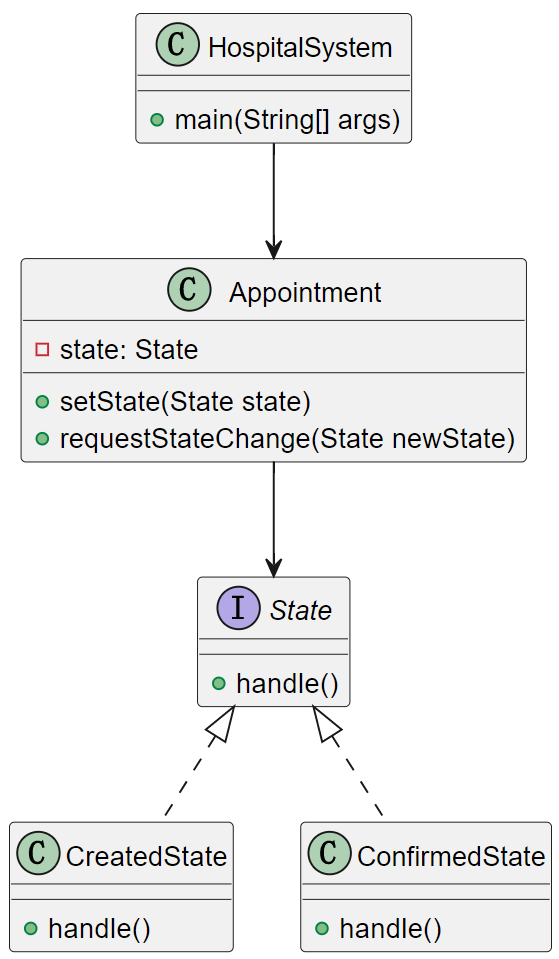
\includegraphics[width=0.4\textheight]{figures/11.png}
	\caption{Builder Pattern}
\end{figure}
在这个例子中,Appointment类作为上下文对象,持有一个State对象的引用,代表当前的预约状态。当需要改变状态时,appointment对象调用requestStateChange方法,并传入新的State对象。新的State对象随后调用handle方法来执行与状态相关的行为。

状态模式在医疗信息系统中的应用,可以使得系统更加灵活地处理各种状态变化,从而为病人提供全面、便捷的医疗服务体验。这包括病人注册登录、查看个人信息、向AI咨询病情、查看医院科室信息、预约挂号、查看可选时段和医生、提交和查询账单、缴纳费用、查询处方以及搜索相关病历等功能。通过这种模式,系统能够及时响应病人的需求和预约状态的变化,提高医疗服务的可及性和效率。


\subsubsection{策略}

策略模式(Strategy Pattern)是一种行为型设计模式,它允许开发者定义一系列算法,并将每个算法封装在独立的类中。这些类实现了一个共同的接口或抽象类,从而使得它们可以互换使用。策略模式的关键在于将算法的变化独立于使用算法的客户,这样客户端代码就可以根据需要灵活地切换不同的策略,而无需修改其本身。

在医疗信息系统中,策略模式可以用于实现提醒策略的多样化和灵活配置。例如,系统可能需要提供不同类型的提醒服务,如短信提醒、邮件提醒、移动应用推送提醒等。每种提醒方式都可以实现为一个策略类,它们都实现了一个共同的提醒接口。医疗信息系统的事件上下文(如预约或检查结果)可以根据病人的偏好或系统的要求,动态地选择和切换不同的提醒策略。

以下是一个简化的代码示例,展示了如何在医疗信息系统中应用策略模式来管理提醒策略:
\begin{lstlisting}[caption={策略模式代码示例}]
% 提醒接口
interface NotificationStrategy {
	void notify(String message);
}

% 短信提醒策略
class SMSNotificationStrategy implements NotificationStrategy {
	@Override
	public void notify(String message) {
		System.out.println("Sending SMS: " + message);
	}
}

% 邮件提醒策略
class EmailNotificationStrategy implements NotificationStrategy {
	@Override
	public void notify(String message) {
		System.out.println("Sending Email: " + message);
	}
}

% 移动应用推送提醒策略
class AppNotificationStrategy implements NotificationStrategy {
	@Override
	public void notify(String message) {
		System.out.println("Sending App Notification: " + message);
	}
}

% 事件上下文
class EventContext {
	private NotificationStrategy strategy;
	
	public void setNotificationStrategy(NotificationStrategy strategy) {
		this.strategy = strategy;
	}
	
	public void sendNotification(String message) {
		strategy.notify(message);
	}
}

% 客户端代码
public class HospitalSystem {
	public static void main(String[] args) {
		EventContext context = new EventContext();
		
		% 设置提醒策略为短信提醒
		context.setNotificationStrategy(new SMSNotificationStrategy());
		context.sendNotification("Your appointment has been confirmed.");
		
		% 切换提醒策略为邮件提醒
		context.setNotificationStrategy(new EmailNotificationStrategy());
		context.sendNotification("Your lab results are ready.");
	}
}

\end{lstlisting}
UML图为:
\begin{figure}[htbp]
	\centering
	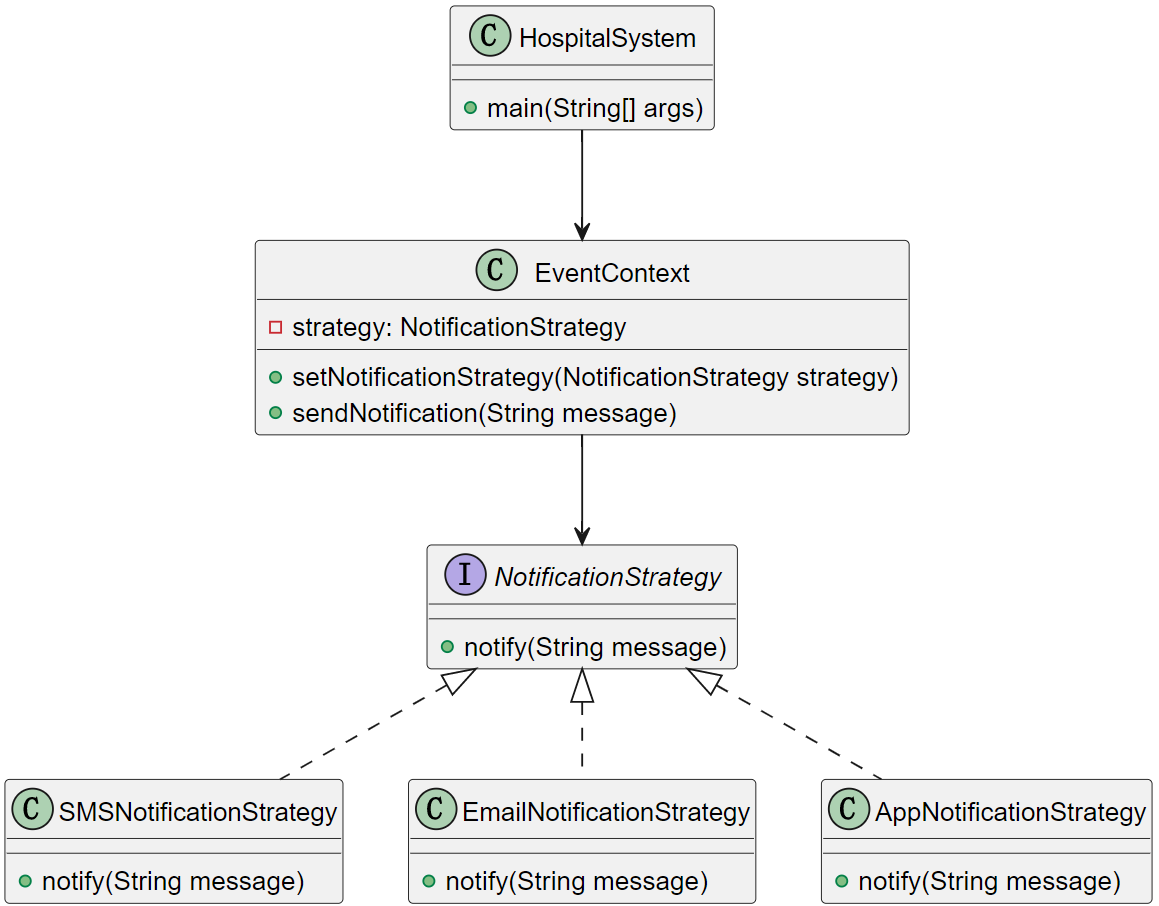
\includegraphics[width=0.4\textheight]{figures/12.png}
	\caption{Builder Pattern}
\end{figure}
在这个例子中,EventContext类作为事件上下文,持有一个NotificationStrategy对象的引用,代表当前的提醒策略。当需要发送提醒时,context对象调用sendNotification方法,并传入提醒信息。不同的提醒策略通过实现NotificationStrategy接口来定义具体的提醒行为。

策略模式在医疗信息系统中的应用,可以使得系统更加灵活地处理提醒服务的配置和变化,从而为病人提供全面、便捷的医疗服务体验。这包括病人注册登录、查看个人信息、向AI咨询病情、查看医院科室信息、预约挂号、查看可选时段和医生、提交和查询账单、缴纳费用、查询处方以及搜索相关病历等功能。通过这种模式,系统能够及时响应病人的需求和提醒策略的变化,提高医疗服务的可及性和效率。

\subsubsection{模版方法}
模板方法模式的核心优势在于它能够确保算法的结构保持不变,同时允许子类根据需要定制算法的某些部分。这种模式非常适合于那些存在多种类似算法或者需要在不同情况下执行不同步骤的场景。通过定义一个抽象类,我们可以为所有相关的子类提供一个共同的模板方法,这些方法包括对各种处理步骤的调用。子类可以强制实现某些步骤,并在需要时覆盖其他步骤,但模板方法本身不会被覆盖。

在医疗信息系统中,模板方法模式可以用于组织和管理各种医疗服务流程。例如,我们可以为不同类型的预约流程创建一个基类,该类定义了一个模板方法,包括对预约流程中的各个步骤的调用,如预约登记、医生分配、时间安排等。对于特定类型的预约,如专家咨询或常规检查,子类可以实现或覆盖基类中的某些步骤,以适应特定的业务需求。

以下是一个简化的代码示例,展示了如何在医疗信息系统中应用模板方法模式来管理预约流程:
\begin{lstlisting}[caption={模版方法示例}]
% 抽象类:预约流程
abstract class AppointmentProcess {
	% 抽象方法,由子类实现具体的预约登记步骤
	protected abstract void registerAppointment();
	
	% 抽象方法,由子类实现具体的医生分配步骤
	protected abstract void allocateDoctor();
	
	% 抽象方法,由子类实现具体的时间安排步骤
	protected abstract void scheduleTime();
	
	% 通用步骤,发送预约确认通知
	private void sendConfirmation() {
		System.out.println("Appointment confirmed and notification sent.");
	}
}

% 专家咨询预约流程的子类
class SpecialistAppointment extends AppointmentProcess {
	@Override
	protected void registerAppointment() {
		System.out.println("Registering specialist appointment request.");
	}
	
	@Override
	protected void allocateDoctor() {
		System.out.println("Allocating specialist doctor.");
	}
	
	@Override
	protected void scheduleTime() {
		System.out.println("Scheduling time for specialist consultation.");
	}
}

% 客户端代码
public class HospitalSystem {
	public static void main(String[] args) {
		SpecialistAppointment specialistAppointment = new SpecialistAppointment();
		specialistAppointment.performAppointment();
	}
}
\end{lstlisting}
UML图为:
\begin{figure}[htbp]
	\centering
	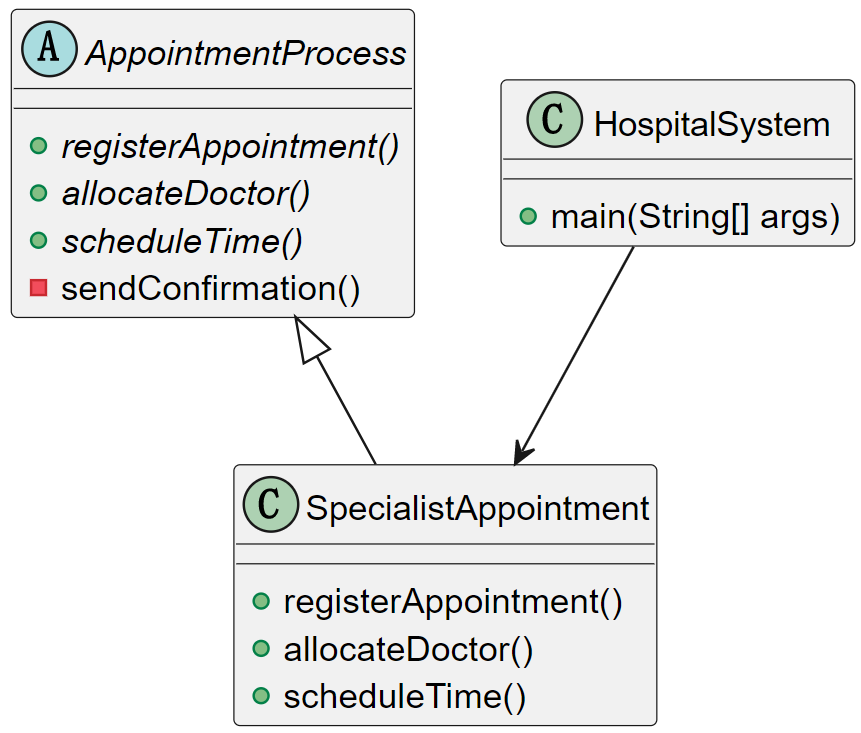
\includegraphics[width=0.4\textheight]{figures/10.png}
	\caption{Builder Pattern}
\end{figure}

在这个例子中,AppointmentProcess类定义了一个模板方法performAppointment,它规定了预约流程的骨架。SpecialistAppointment类作为子类,实现了针对专家咨询预约的具体步骤。当调用performAppointment方法时,它会按照定义的顺序执行所有步骤,包括那些由子类实现的步骤和基类中的通用步骤。

模板方法模式在医疗信息系统中的应用,可以提高医疗服务流程的标准化和可维护性,同时允许针对不同情况定制流程。这有助于为病人提供全面、便捷的医疗服务体验,包括病人注册登录、查看信息、向AI咨询病情、查看科室、预约挂号、查看可选时段和医生、提交和查询账单、缴纳费用、查询处方以及搜索相关病历等功能。通过这种模式,系统能够确保医疗服务的高效性和一致性,同时满足病人的个性化需求。

